\objectives{%
    \item write a simple, inefficient image classifier %ying ML program
    \item visualize data as lying in feature space; visualize hypotheses as
            functions defined on feature space; and visualize the class of
            all hypotheses within weight space
}

%%\samsection{a tiny example: handwritten digit classification}
%      \samquote{
%        The learning process is something you can incite, literally incite, like a riot.
%      }{audre lorde}

%~~~~~~~~~~~~~~~~~~~~~~~~~~~~~~~~~~~~~~~~~~~~~~~~~~~~~~~~~~~~~~~~~~~~~~~~~~~~~~
%~~~~~~~~~~~~~  1.3. meeting the data  ~~~~~~~~~~~~~~~~~~~~~~~~~~~~~~~~~~~~~~~~

\sampassage{meeting the data}
  Say we want to classify handwritten digits.
  In symbols: we'll map $\xX$ to $\yY$ with $\xX =
  \{\text{grayscale~}28\!\times\!28\text{-pixel images}\}$,
  $\yY=\{{\blu{1}},{\rng{3}}\}$.
  Each datum $(x,y)$ arises as follows: we randomly choose a digit $y\in \yY$,
  ask a human to write that digit in pen, and then photograph their writing to
  produce $x\in\xX$.
  %
  \newcommand{\mnistex}[2]{%
      \includegraphics[width=0.75cm]{example-mnist/mnist-trn-#1}\vspace{-0.2cm}%
      \\#2%
  }
  \vspace{-0.25cm}
  \begin{figure}
      \centering
    \vspace{+0.15cm}%
    \begin{tabular}{c}\mnistex{00}{$\rng{3}$}\\\mnistex{10}{$\rng{3}$}\end{tabular}%
    \begin{tabular}{c}\mnistex{01}{$\blu{1}$}\\\mnistex{11}{$\blu{1}$}\end{tabular}%
    \begin{tabular}{c}\mnistex{02}{$\rng{3}$}\\\mnistex{12}{$\rng{3}$}\end{tabular}%
    \begin{tabular}{c}\mnistex{03}{$\rng{3}$}\\\mnistex{13}{$\blu{1}$}\end{tabular}%
    \begin{tabular}{c}\mnistex{04}{$\rng{3}$}\\\mnistex{14}{$\rng{3}$}\end{tabular}%
    \begin{tabular}{c}\mnistex{05}{$\blu{1}$}\\\mnistex{15}{$\blu{1}$}\end{tabular}%
    \begin{tabular}{c}\mnistex{06}{$\blu{1}$}\\\mnistex{16}{$\rng{3}$}\end{tabular}%
    \begin{tabular}{c}\mnistex{07}{$\rng{3}$}\\\mnistex{17}{$\blu{1}$}\end{tabular}%
    \begin{tabular}{c}\mnistex{08}{$\rng{3}$}\\\mnistex{18}{$\rng{3}$}\end{tabular}%
    \begin{tabular}{c}\mnistex{09}{$\rng{3}$}\\\mnistex{19}{$\blu{1}$}\end{tabular}%
    \caption{%
      Twenty example pairs.  Each photo $x$ is a $28\times 28$ grid of
      numbers representing pixel intensities.  The light gray background
      has intensity $0.0$; the blackest pixels, intensity $1.0$.  Below
      each photo $x$ we display the corresponding label $y$:
      either $y= {\blu{1}}$ or
      $y={\rng{3}}$.
      %
      We'll adhere to this color code throughout this tiny example.
    }
  \end{figure}

  \begin{marginfigure}[2.5cm]
    \center
    
\includegraphics[width=0.45\textwidth]{example-mnist/mnist-trn-01}%
    \hspace{0.5cm}%
    
\includegraphics[width=0.45\textwidth]{example-mnist/mnist-trn-00}%
  \end{marginfigure}
  When we zoom in, we can see each photo's $28\times 28$ grid of pixels.
  On the computer, this data is stored as a $28\times 28$ grid of
  numbers: $0.0$ for bright through $1.0$ for dark.  We'll name these
  $28\times28$ grid locations by their row number (counting from
  the top) followed by their column number (counting from the
  left).  So location $(0,0)$ is the upper left corner pixel;
  $(27,0)$, the lower left corner pixel.
  \par\noindent
  \exercise{Where is location $(0,27)$?  %$(14,8)$?
  Which way is $(14,14)$ off-center?}

  To get to know the data, let's wonder how we'd hand-code a
  classifier (worry not: soon we'll do this more automatically).
  We want to complete the code
  %
  \begin{lstlisting}[language=Python, basicstyle=\footnotesize\ttfamily]
    def hand_coded_predict(x):
      return 3 if condition(x) else 1
  \end{lstlisting}
  %
  Well, ${\rng{3}}$s tend to have more ink than than ${\blu{1}}$s ---
  should \texttt{condition}\ threshold by the photo's brightness?
  %
  Or: ${\blu{1}}$s and ${\rng{3}}$s tend to have different widths ---
  should \texttt{condition}\ threshold by the photo's dark part's width?

  To make this precise, let's define a photo's \emph{brightness} as $1.0$ minus
  its average pixel darkness; its \emph{width} as the standard deviation of
  the column index of its dark pixels.
    Such
  functions from inputs in $\xX$ to numbers are called
  \textbf{features}.
      %return np.mean(np.mean(x, axis=0), axis=0)
  \begin{lstlisting}[language=Python, basicstyle=\footnotesize\ttfamily]
    SIDE = 28
    def brightness(x):  return 1. - np.mean(x)
    def width(x):       return np.std([col for col in range(SIDE)
                                           for row in range(SIDE)
                                           if 0.5 < x[row][col]  ])/(SIDE/2.0)
    # (we normalized width by SIDE/2.0 so that it lies within [0., 1.]) 
  \end{lstlisting}
  %\par\noindent
  %\begin{figure}[h]
  \begin{marginfigure}[-2.5cm]
    \centering
    %\vspace{-3.5cm}
    %
\includegraphics[width=0.24\textwidth]{example-mnist/mnist-trn-00}
    %
\includegraphics[width=0.24\textwidth]{example-mnist/mnist-trn-01}
    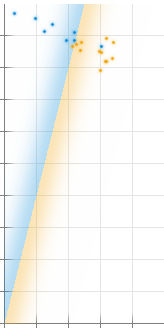
\includegraphics[width=0.85\textwidth]{example-mnist/train-plain-cropped}
    \caption{%
      \textbf{Featurized training data.}
      Our $N=20$ many training examples, viewed in the
      brightness-width plane.  The vertical \emph{brightness} axis ranges
      $[0.0,1.0]$; the horizontal \emph{width} axis ranges $[0.0,0.5]$.
      The origin is at the lower left.  {\rng{Orange}} dots represent
      $y={\rng{3}}$ examples; {\blu{blue}} dot, $y={\blu{1}}$ examples.
      %
      We eyeballed the line $-1\cdot \text{brightness} +4\cdot\text{width}=0$
      to separate the two kinds of examples.
      %
      %The big ${\rng{3}}$ above has brightness and width $(0.118, 0.375)$;\
      %the big ${\blu{1}}$, $(0.092, 0.404)$.  See where they are in this
      %plot?
    }
  \end{marginfigure}
  %\end{figure}

  So we can threshold by brightness or by width.  But this isn't very
  satisfying, since sometimes there are especially dark ${\blu{1}}$s or
  thin ${\rng{3}}$s.
  %
  Aha!  Let's use \emph{both} features: ${\rng{3}}$s are darker than
  ${\blu{1}}$s \emph{even relative to their width}.  Inspecting the
  training data, we see that a line through the origin of slope $4$
  roughly separates the two classes.  So let's
  threshold by a combination like \texttt{-1*brightness(x)+4*width(x)}:
  %\bovinenote{%
  %  \blarr That factor of $2$ comes from our observation that brightness
  %  tends to be bigger than width.  We'll soon see that this eyeballed
  %  slope doesn't work well.  It's better to tune by machine.
  %}
  \begin{minipage}{\linewidth}
  \begin{lstlisting}[language=Python, basicstyle=\footnotesize\ttfamily]
    def condition(x):
      return -1*brightness(x)+4*width(x) > 0
  \end{lstlisting}
  \end{minipage}
  Intuitively, the formula $-1\cdot \text{brightness} +4\cdot\text{width}$ we
  invented is a measure of \emph{threeness}: if it's positive, we predict
  $y={\rng 3}$.  Otherwise, we predict $y={\blu 1}$.
  %\exercise{Guess a good pair $(a,b)$ based on the training data.}
  %\exercise{Implement a crude ``hole-detector'' feature.  False positives are
  %okay.}
  %\exercise{Make a width feature.  Plot the training data in the
  %width-width plane.}
  \exercise{%
      What further features might help us separate digits
        ${\blu{1}}$ from ${\rng{3}}$?
  }



\pagebreak
\sampassage{candidate patterns}
  We can generalize the hand-coded hypothesis from the previous passage
  to other coefficients besides $-1\cdot \text{brightness}(x) +4\cdot\text{width}(x)$.  We let our set $\hH$ of candidate patterns
  contain all ``linear hypotheses'' $f_{a,b}$ defined by:
  $$
    f_{a,b}(x) = {\rng{3}} \text{~~if~~} a\cdot\text{brightness}(x) + b\cdot\text{width}(x) > 0 \text{~~else~~} {\blu{1}}
  $$
  Each $f_{a,b}$ makes predictions of $y$s given $x$s.  As we change $a$
  and $b$, we get different predictors, some more accurate than others.
  \begin{marginfigure}[-0.0cm]
      \centering
      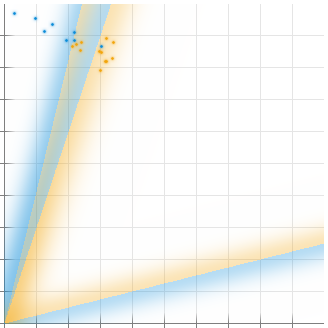
\includegraphics[width=0.99\textwidth]{example-mnist/train-features.png}%
      %
      \caption{%
        \textbf{Hypotheses differ in training accuracy: feature space.}
        %
        $3$ hypotheses classify training data in the brightness-width
        plane (axes range $[0, 1.0]$).
        Glowing colors distinguish a
        hypothesis' $\blu{1}$ and $\rng{3}$ sides.
        For instance, the bottom-most line classifies all the training points
        as $\rng{3}$s.
        %
        \textbf{Caution}: the colors in this page's two Figures
        represent unrelated distinctions!
      }
      \label{fig:train-features}
  \end{marginfigure}

  \begin{lstlisting}[language=Python, basicstyle=\footnotesize\ttfamily]
    def predict(x,a,b):
      return 3 if a*brightness(x) + b*width(x) > 0 else 1
  \end{lstlisting}
  The brightness-width plane is called \textbf{feature space}: its points
  represent inputs $x$ in terms of chosen features (here, brightness and
  width).  The $(a,b)$ plane is called \textbf{weight space}: its points
  represent linear hypotheses $h$ in terms of the coefficients --- or \textbf{weights} ---
  $h$ places on each feature (e.g. $a=-1$ on brightness and $b=+4$ on width).

  \exercise{Which of Fig.\ \ref{fig:train-features}'s $3$ hypotheses best predicts training data?
  }

  \exercise{What $(a,b)$ pairs might have produced Fig.\
  \ref{fig:train-features}'s $3$ hypotheses?  Can you determine $(a,b)$
  for sure, or is there ambiguity (i.e., can multiple $(a,b)$ pairs make
  exactly the same predictions in brightness-width space)?
  }

%~~~~~~~~~~~~~~~~~~~~~~~~~~~~~~~~~~~~~~~~~~~~~~~~~~~~~~~~~~~~~~~~~~~~~~~~~~~~~~
%~~~~~~~~~~~~~  1.5. optimization  ~~~~~~~~~~~~~~~~~~~~~~~~~~~~~~~~~~~~~~~~~~~~

\sampassage{optimization}
  Let's write a program to automatically find hypothesis $h=(a,b)$ from the
  training data.  We want to predict the labels $y$ of yet-unseen photos $x$
  (\emph{testing examples}); insofar as training data is representative of
  testing data, it's sensible to return a $h\in \hH$ that correctly classifies
  maximally many training examples.

  %%Let's write a program $\lL$ that given a list of \emph{training
  %%examples} produces a hypothesis in $h \in \hH$ that helps us predict
  %%the labels $y$ of yet-unseen photos $x$ (\emph{testing examples}).
  %%Insofar as training data is representative of testing data, it's
  %%sensible to return a $h\in \hH$ that correctly classifies maximally
  %%many training examples.
  %
  To do this, let's just loop over a bunch $(a,b)$s --- say, all integer
  pairs in $[-99,+99]$ --- and pick one that misclassifies the least
  training examples:
  \begin{lstlisting}[language=Python, basicstyle=\footnotesize\ttfamily]
    def is_correct(x,y,a,b):
      return 1.0 if predict(x,a,b)==y else 0.0
    def accuracy_on(examples,a,b):
      return np.mean(is_correct(x,y,a,b) for x,y in examples)
    def best_hypothesis():
      # returns a pair (accuracy, hypothesis)
      return max((accuracy_on(training_data, a, b), (a,b))
                 for a in np.arange(-99,+100)
                 for b in np.arange(-99,+100)             )
  \end{lstlisting}

  %%\begin{figure}[h]
  \begin{marginfigure}[-2.2cm]
      \centering
      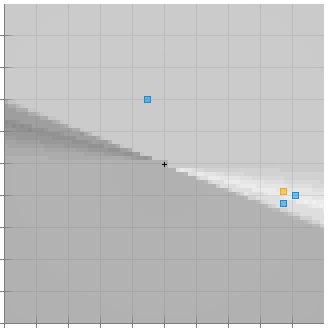
\includegraphics[width=0.99\textwidth]{example-mnist/train-weights.png}\\%
      %
      \caption{%
        \textbf{Hypotheses differ in training accuracy: weight space.}
        %
        We visualize $\hH$ as the $(a,b)$-plane (axes range
        $[-99,+99]$).  Each point determines a whole line in the
        brightness-width plane.  Shading shows training error: darker points
        misclassify more training examples.  The least shaded, most training-accurate
        hypothesis is $(-20, 83)$: the rightmost of the $3$
        {\blu blue squares}.
        %
        The {\rng orange square} is the hypothesis that best fits our unseen
        testing data.
        %--- in the real world we can't compute it but in this toy
        %example we can.
        %
        %
        %\par\noindent
    \exercise{Suppose Fig.\ \ref{fig:train-features}'s $3$ hypotheses arose
    from Fig.\ \ref{fig:train-weights}'s $3$ {\blu blue squares}.
    Which hypothesis matches each square?}
      }
      \label{fig:train-weights}
  \end{marginfigure}



%(0, -2.0, 8.25) reduces train error to 0.10; has test error 0.17
%(0, -1.75, 7.5) reduces test error to 0.15; has train error 0.15

  Fed our $N=20$ training examples, the loop finds
  $(a,b)=(-20,+83)$ as a minimizer of \textbf{training error}, i.e.,
  of the fraction of training examples misclassified.  It misclassifies
  only $10\%$ of training examples. Yet the same
  hypothesis misclassifies a greater fraction --- $17\%$ --- of fresh,
  yet-unseen testing examples.
  %
  That latter number --- called the \textbf{testing error} --- represents
  our program's accuracy ``in the wild''; it's the number we most care
  about.

  The difference between training and testing error is the
  difference between our score on our second try on a practice exam (after we've reviewed
  our mistakes) versus our score on a real
  exam (where we don't know the questions beforehand and aren't allowed
  to change our answers once we get our grades back).

      \exercise{In the $(a,b)$ plane shaded by training error, we see two
  `cones', one dark and one light.  They lie geometrically opposite to each
      other --- why?}

  \exercise{Sketch $f_{a,b}$'s error on $N=1$ example as a
  function of $(a,b)$.}


%    
\includegraphics[width=0.75cm]{example-mnist/mnist-trn-10}\vspace{-0.2cm}\\$\blu{1}$\end{tabular}%
%    \begin{tabular}{c}
\includegraphics[width=0.75cm]{example-mnist/mnist-trn-01}\vspace{-0.2cm}\\$\blu{1}$\\
\includegraphics[width=0.75cm]{example-mnist/mnist-trn-11}\vspace{-0.2cm}\\$\rng{3}$\end{tabular}%
%    \begin{tabular}{c}
\includegraphics[width=0.75cm]{example-mnist/mnist-trn-02}\vspace{-0.2cm}\\$\rng{3}$\\
\includegraphics[width=0.75cm]{example-mnist/mnist-trn-12}\vspace{-0.2cm}\\$\blu{1}$\end{tabular}%
%    \begin{tabular}{c}
\includegraphics[width=0.75cm]{example-mnist/mnist-trn-03}\vspace{-0.2cm}\\$\rng{3}$\\
\includegraphics[width=0.75cm]{example-mnist/mnist-trn-13}\vspace{-0.2cm}\\$\blu{1}$\end{tabular}%
%    \begin{tabular}{c}
\includegraphics[width=0.75cm]{example-mnist/mnist-trn-04}\vspace{-0.2cm}\\$\blu{1}$\\
\includegraphics[width=0.75cm]{example-mnist/mnist-trn-14}\vspace{-0.2cm}\\$\rng{3}$\end{tabular}%
%    \begin{tabular}{c}
\includegraphics[width=0.75cm]{example-mnist/mnist-trn-05}\vspace{-0.2cm}\\$\rng{3}$\\
\includegraphics[width=0.75cm]{example-mnist/mnist-trn-15}\vspace{-0.2cm}\\$\rng{3}$\end{tabular}%
%    \begin{tabular}{c}
\includegraphics[width=0.75cm]{example-mnist/mnist-trn-06}\vspace{-0.2cm}\\$\rng{3}$\\
\includegraphics[width=0.75cm]{example-mnist/mnist-trn-16}\vspace{-0.2cm}\\$\rng{3}$\end{tabular}%
%    \begin{tabular}{c}
\includegraphics[width=0.75cm]{example-mnist/mnist-trn-07}\vspace{-0.2cm}\\$\rng{3}$\\
\includegraphics[width=0.75cm]{example-mnist/mnist-trn-17}\vspace{-0.2cm}\\$\blu{1}$\end{tabular}%
%    \begin{tabular}{c}
\includegraphics[width=0.75cm]{example-mnist/mnist-trn-08}\vspace{-0.2cm}\\$\blu{1}$\\
\includegraphics[width=0.75cm]{example-mnist/mnist-trn-18}\vspace{-0.2cm}\\$\rng{3}$\end{tabular}%
%    \begin{tabular}{c}
\includegraphics[width=0.75cm]{example-mnist/mnist-trn-09}\vspace{-0.2cm}\\$\rng{3}$\\
\includegraphics[width=0.75cm]{example-mnist/mnist-trn-19}\vspace{-0.2cm}\\$\blu{1}$\end{tabular}%
%


